\mode*

\begin{frame}
  \frametitle{Implementierung}
  \begin{itemize}
    \item Programmiersprache: C++
      \begin{itemize}
        \item Speichereffizienz, Performanz und leichte Anbindung an bestehende Frameworks
      \end{itemize}
    \item Realisierung als statische Bibliothek
      \begin{itemize}
        \item erm\"oglicht bequeme Einbindung in den Linking-Prozess
        \item es m\"ussen nur Bibliotheksdatei und Header-Dateien zur Verf\"ugung stehen
      \end{itemize}
  \end{itemize}
\end{frame}

\begin{frame}
  \frametitle{Implementierung}
  \begin{figure}
    \centering
    \resizebox{0.9\textwidth}{!}{\begin{tikzpicture}%[show background grid]
      \begin{class}[text width=15cm]{Propagator}{0,0}
        \attribute{- fieldDescriptor: FieldDescriptor}

        \operation{+ Propagator( fieldDescriptor: FieldDescriptor )}
        \operation{+ getTrack( particle: Particle, stoppingCondition: Condition, initialTimeStep: double ): vector<Particle>}
      \end{class}

      \begin{interface}[text width=7.5cm]{FieldDescriptor}{-4, -4}
        \operation{getStrength( location: Vector3D ): Vector3D}
      \end{interface}
      
      \begin{interface}[text width=6.5cm]{Condition}{4, -4}
        \operation{check( track: vector<Particle> ): bool}
      \end{interface}

      \begin{class}[text width=6cm]{MaximumDistanceCondition}{-4, -7}
        \implement{Condition}
        \attribute{- maxDistance: double}
        \attribute{- referencePoint: Vector3D}
      \end{class}

      \begin{class}[text width=6cm]{PlaneIntersectionCondition}{4, -7}
        \implement{Condition}
        \attribute{- plane: Plane3D}
      \end{class}

      \draw[umlcd  style  dashed  line ,->] (Propagator) --node[above , sloped ,
        black]{} (FieldDescriptor);

      \draw[umlcd  style  dashed  line ,->] (Propagator) --node[above , sloped ,
        black]{} (Condition);
    \end{tikzpicture}}
    \caption{Die strukturelle Anordnung der wichtigsten Klassen und Schnittstellen.}
    \label{fig:klassen}
  \end{figure}
\end{frame}

\begin{frame}
  \frametitle{Implementierung}
  \textbf{Verwendete Entwicklerwerkzeuge}
  \begin{itemize}
    \item CMake (Cross-Platform Make)
      \begin{itemize}
        \item erkennt automatisch Abh\"angigkeiten zwischen den Quelldateien
        \item kann automatisch Makefiles erzeugen (auf Windows auch Visual Studio Projekte)
        \item erm\"oglicht unabh\"angige Verarbeitung von Softwarekomponenten
          \begin{itemize}
            \item getrenntes \"Ubersetzen von Testf\"allen und Demonstrationsf\"allen
          \end{itemize}
      \end{itemize}
    \item Google Test
      \begin{itemize}
        \item Unittest-Prinzip
        \item unabh\"angige Testf\"alle unabh\"angiger Komponenten
        \item leichte Durchf\"uhrung von Regressionstests
      \end{itemize}
    \item Gnuplot
      \begin{itemize}
        \item eingesetzt zur Visualisierung der Demonstrationsf\"alle
      \end{itemize}
  \end{itemize}
\end{frame}

\begin{frame}
  \frametitle{Implementierung}
  \begin{figure}
    \centering
    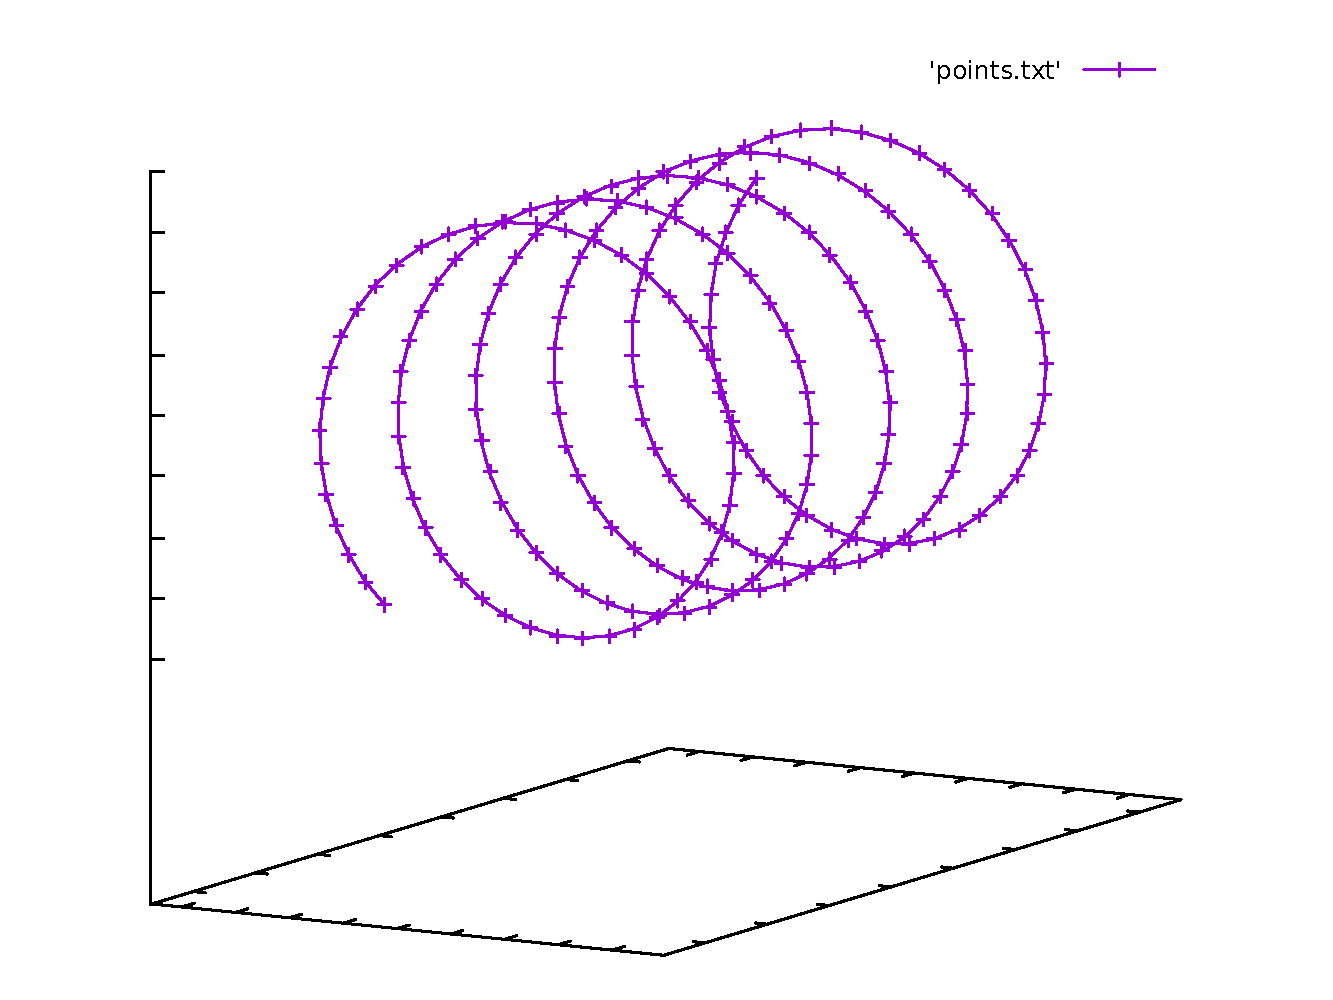
\includegraphics[width=0.6\textwidth]{../gnuplot/homogeneous}
    \caption{Die Schraubenlinien der Teilchenbewegung im homogenen Magnetfeld.}
    \label{fig:homogeneous_plot}
  \end{figure}
\end{frame}

\begin{frame}
  \frametitle{Implementierung}
  \begin{figure}
    \centering
    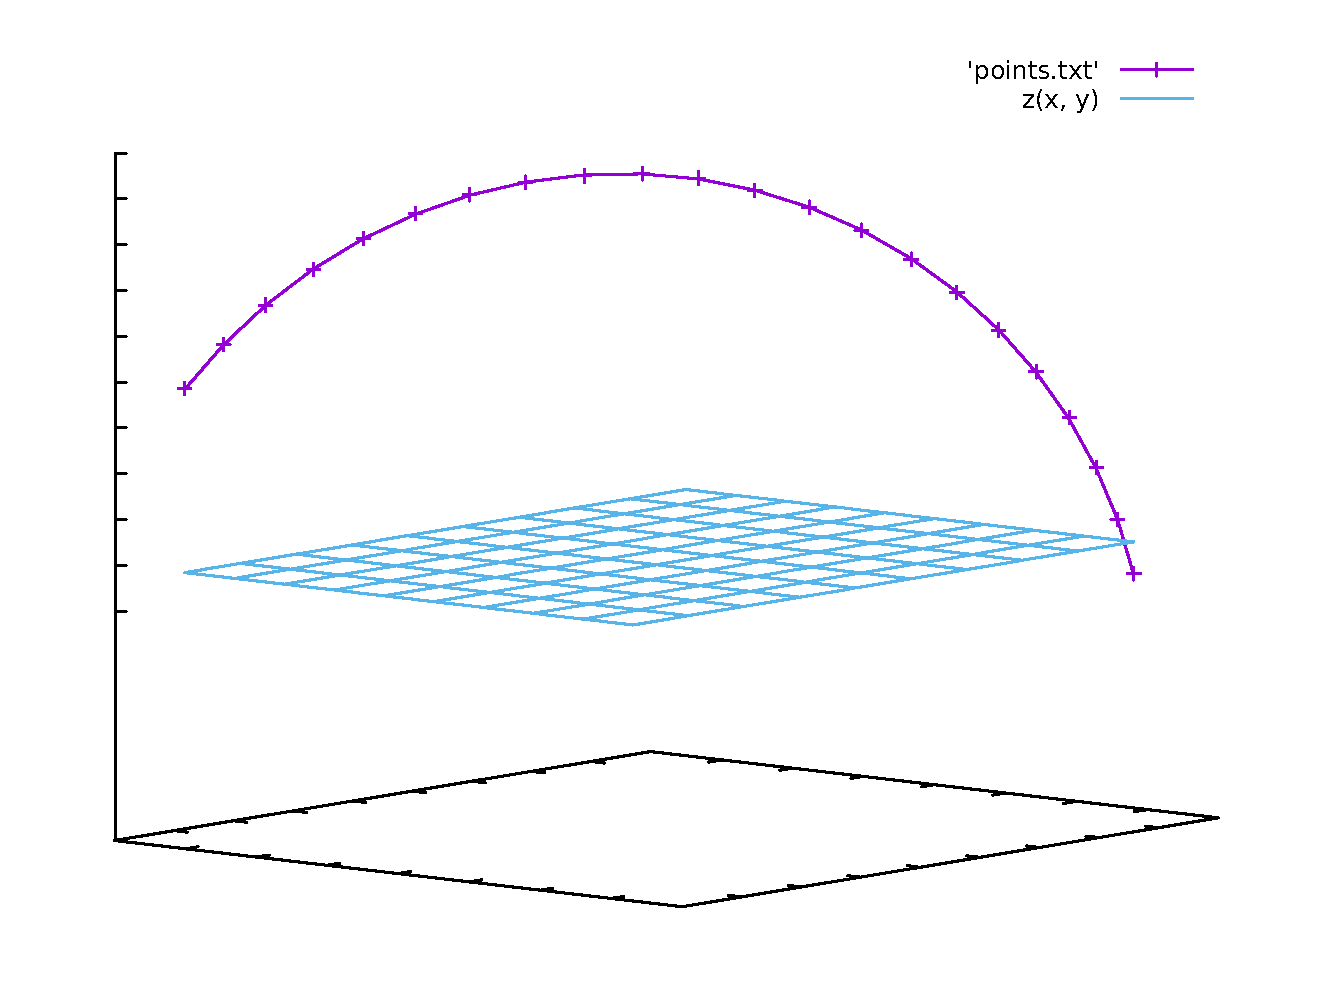
\includegraphics[width=0.6\textwidth]{../gnuplot/stop_plane}
    \caption{Die Simulation wird beendet, sobald das Teilchen die Ebene durchquert.}
    \label{fig:stop_plane}
  \end{figure}
\end{frame}

\begin{frame}
  \frametitle{Implementierung}
  \begin{figure}
    \centering
    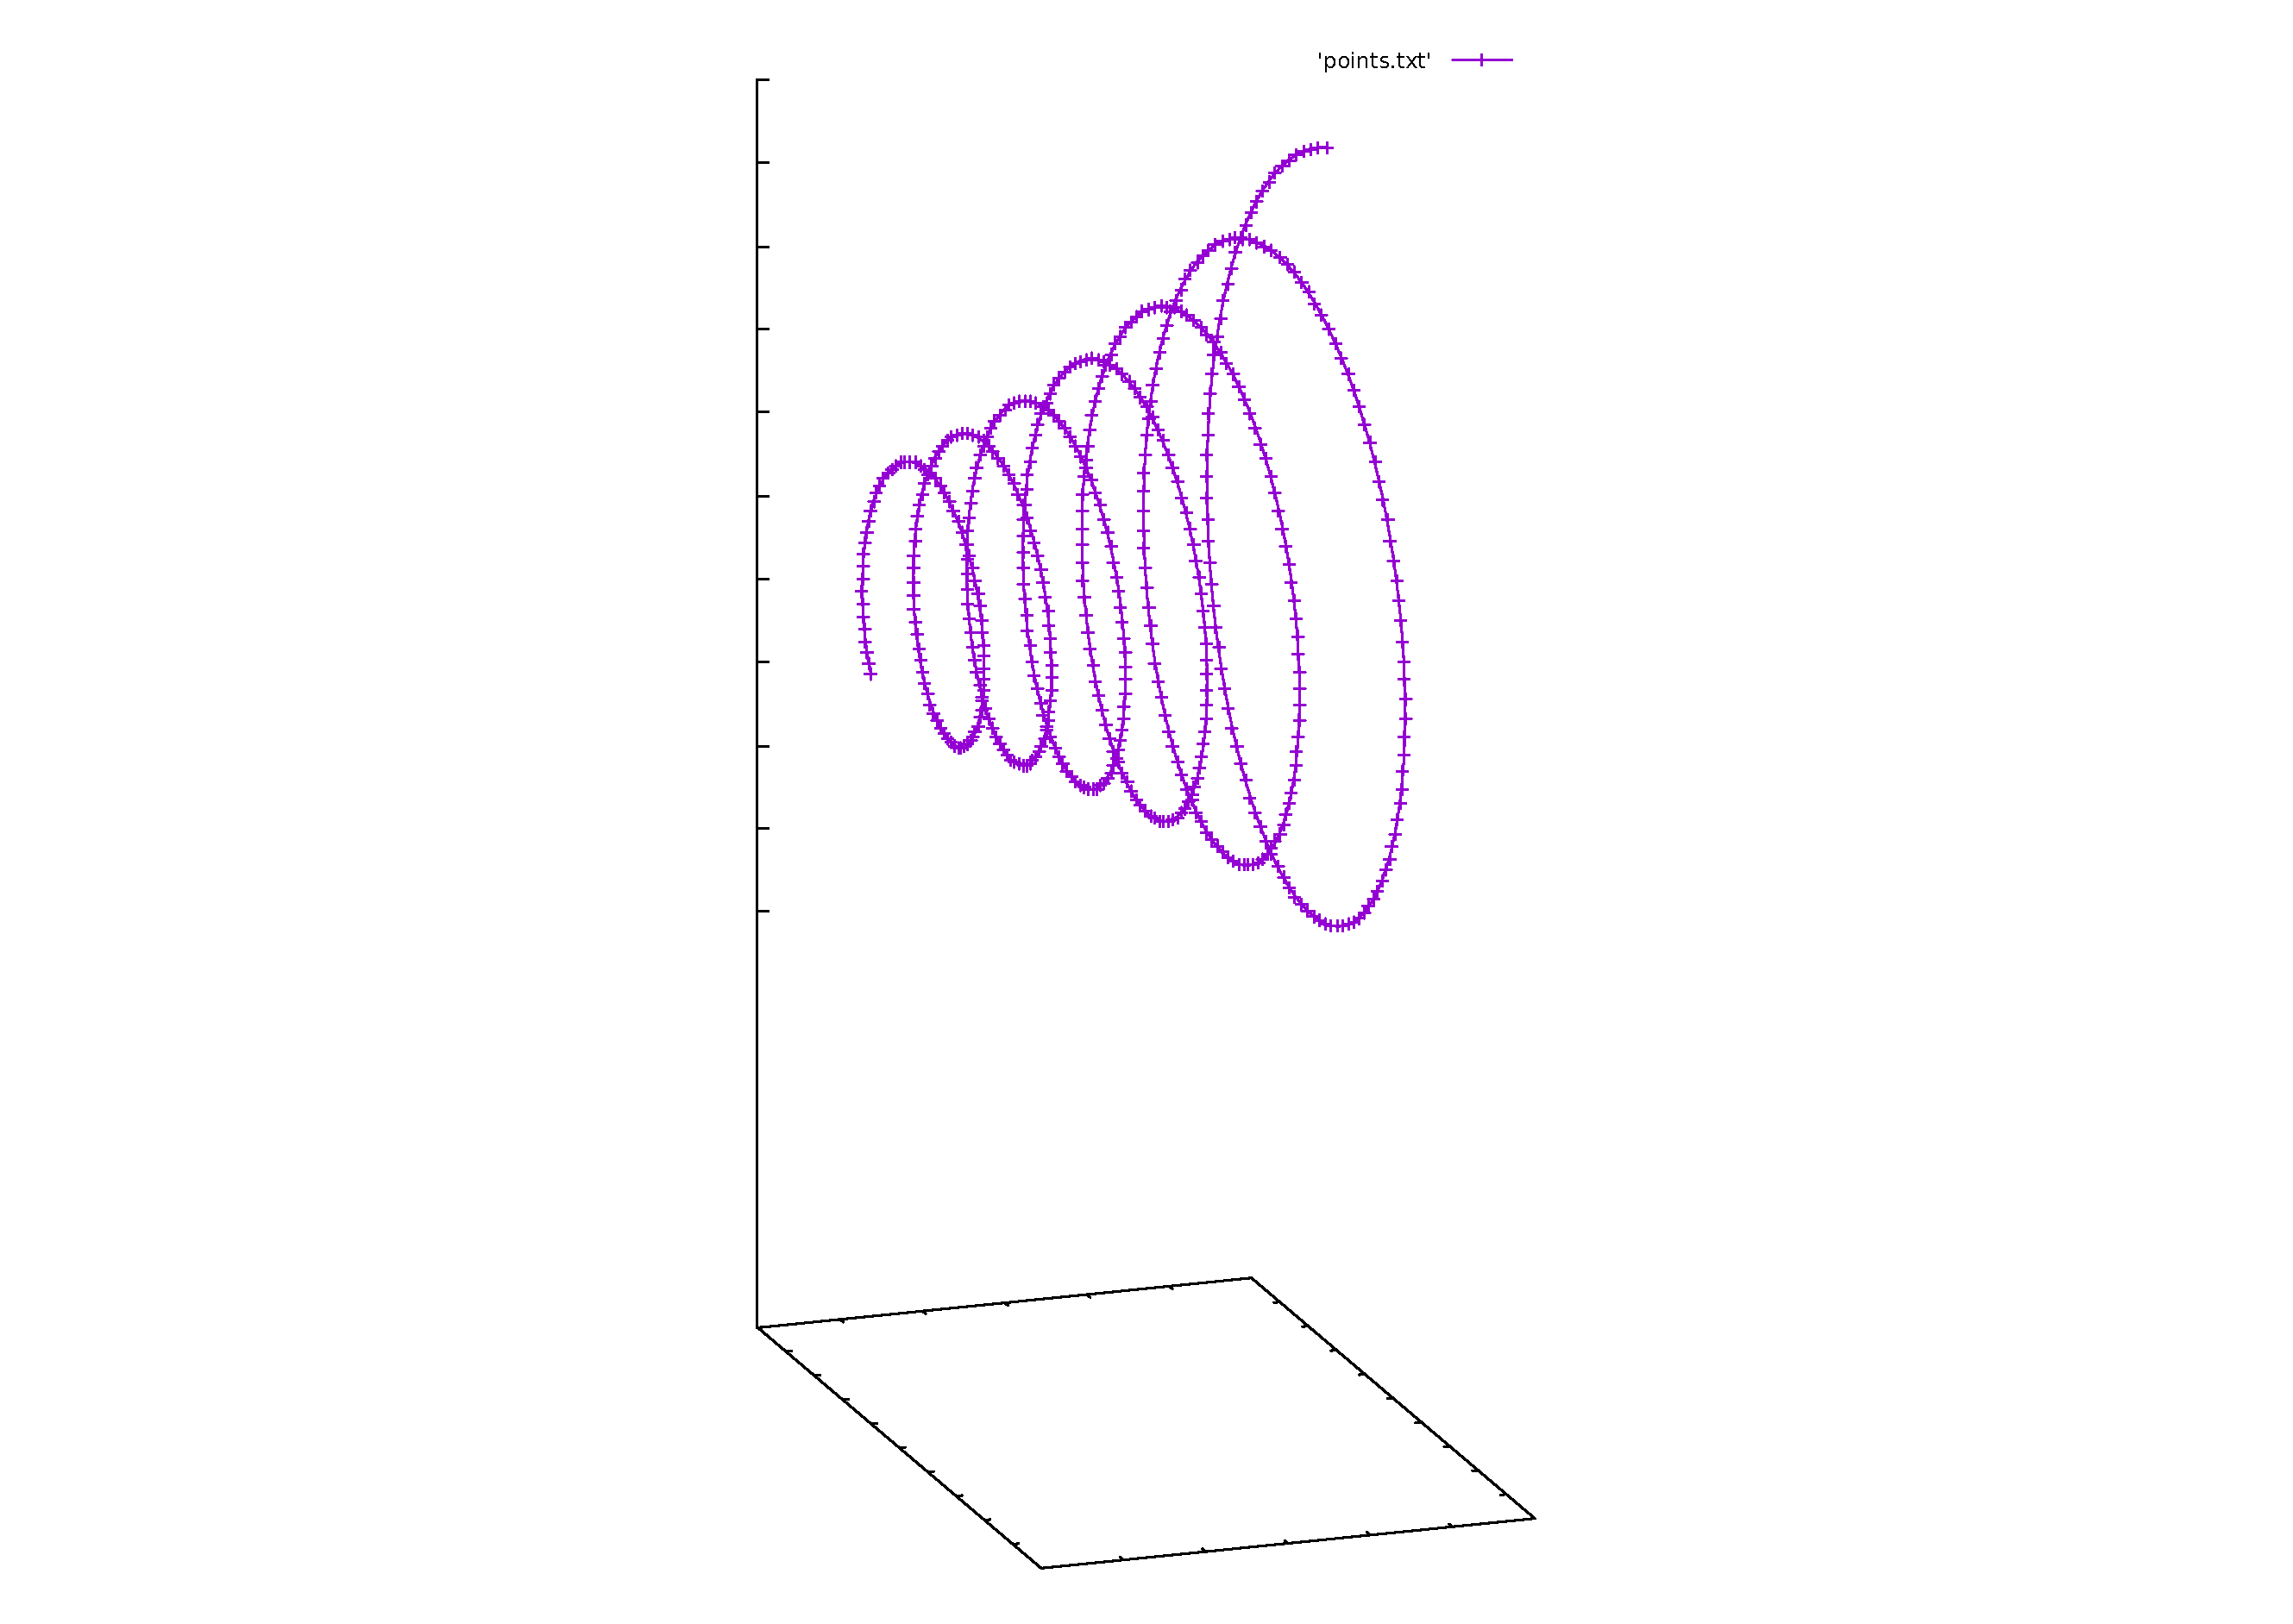
\includegraphics[width=0.7\textwidth]{../gnuplot/fading_field}
    \caption{Die exponentiell abnehmende Feldst\"arke f\"uhrt zu einer Vergr\"o{\ss}erung des Radius.}
    \label{fig:fading_field}
  \end{figure}
\end{frame}

\mode<all>
